\documentclass[11pt,a4paper]{article}
\usepackage[utf8]{inputenc}
\usepackage[spanish,es-tabla]{babel}
\usepackage{amsmath}
\usepackage{amsfonts}
\usepackage{amssymb}
\usepackage{geometry}
\usepackage{xcolor}
\usepackage{titlesec}
\usepackage{booktabs}
\usepackage{enumitem}
\usepackage{microtype}
\usepackage{listings}
\usepackage{graphicx}
\usepackage{hyperref}

% --- Configuración de Márgenes Estrictos de Documentación Académica ---
\geometry{top=2.5cm, bottom=2.5cm, left=3cm, right=2.5cm}

% --- Paleta de Colores Corporativa para Entornos de Desarrollo ---
\definecolor{teincoblue}{RGB}{23, 32, 42}       % Azul Oscuro de Consola
\definecolor{accentblue}{RGB}{41, 128, 185}     % Azul de Enfoque Algorítmico
\definecolor{emeraldideal}{RGB}{22, 160, 133}   % Verde Menta para Hilos de Ejecución
\definecolor{lightgray}{RGB}{245, 247, 250}

% --- Estilizado de Títulos Dinámicos ---
\titleformat{\section}{\color{teincoblue}\normalfont\large\bfseries}{\thesection}{1em}{}
\titleformat{\subsection}{\color{accentblue}\normalfont\normalsize\bfseries}{\thesubsection}{1em}{}
\titleformat{\subsubsection}{\color{teincoblue}\normalfont\normalsize\itshape}{\thesubsubsection}{1em}{}

% CONFIGURACIÓN EXTENDIDA DE LISTINGS PARA SOPORTAR UTF-8 (TILDES)
\lstset{
	backgroundcolor=\color{lightgray},
	basicstyle=\small\ttfamily,
	breaklines=true,
	keywordstyle=\color{accentblue}\bfseries,
	frame=single,
	showstringspaces=false,
	extendedchars=true,
	literate={á}{{\'a}}1 {é}{{\'e}}1 {í}{{\'i}}1 {ó}{{\'o}}1 {ú}{{\'u}}1 {ñ}{{\~n}}1 {Á}{{\'A}}1 {É}{{\'E}}1 {Í}{{\'I}}1 {Ó}{{\'O}}1 {Ú}{{\'U}}1 {Ñ}{{\~N}}1 {ú}{{\'u}}1
}

\hypersetup{
	colorlinks=true,
	linkcolor=teincoblue,
	filecolor=accentblue,      
	urlcolor=accentblue,
	citecolor=emeraldideal
}

\begin{document}
	
	% ==========================================
	% PORTADA TÉCNICA E INSTITUCIONAL (DESARROLLADOR)
	% ==========================================
	\begin{titlepage}
		\centering
		\vspace*{1cm}
		{\large\bfseries CORPORACIÓN TECNOLÓGICA INDUSTRIAL COLOMBIANA - TEINCO} \\[0.3cm]
		{\large FACULTAD DE INGENIERÍA DE SISTEMAS} \\[2.5cm]
		
		{\color{teincoblue}\Huge\bfseries MANUAL TÉCNICO DE INGENIERÍA DE SOFTWARE Y COMPENDIO DE CÓDIGO FUENTE} \\[0.8cm]
		{\color{accentblue}\Large\bfseries Arquitectura, Patrones de Diseño y Modelamiento Numérico del Multi-Ecosistema} \\[0.5cm]
		{\large\bfseries Guía Avanzada de Desarrollo: Motor Gráfico, Simulación Física e Hilos de Trabajo} \\[1cm]
		{\normalsize\bfseries Versión del Núcleo v2.1.0 (Rama de Producción)} \\[2.5cm]
		
		\textbf{Línea de Investigación y Código:} \\
		Laura Vanessa Ramírez Baquero \\
	
		\textbf{Área de Desarrollo:} \\
		Estructuras de Datos, Computación Gráfica y Física Matemática Discreta \\[1.5cm]
		
		\textbf{Docente Revisor de Código:} \\
		Prof. Rafael \\[2cm]
		
		\vfill
		{\large Bogotá D.C., Colombia \\ Mayo de 2026}
	\end{titlepage}
	
	% SOLUCIÓN AL IDENTIFIER DUPLICATE: Usar alph para las páginas previas o vaciar el estilo
	\pagenumbering{Alph}
	\tableofcontents
	\clearpage
	
	% Inicialización de numeración arábiga para el cuerpo técnico del manual
	\pagenumbering{arabic}
	
	% ==========================================
	% SECCIÓN 1: INTRODUCCIÓN AL DESARROLLADOR
	% ==========================================
	\section{Introducción Técnico al Núcleo de Simulación}
	El presente documento constituye el compendio técnico de ingeniería y documentación del código fuente del multi-ecosistema de simulación virtual desarrollado para la Corporación Tecnológica Industrial Colombiana (TEINCO). La plataforma está concebida bajo un enfoque de desarrollo modular y programación orientada a objetos (POO) pura utilizando el lenguaje interpretado Java. El sistema encapsula dos componentes core independientes y desacoplados a nivel de lógica de dominio: el motor numérico cinemático para la resolución del \textbf{Módulo I (Tiro Parabólico con Fricción Aerodinámica)} y el solvedor analítico/numérico para el \textbf{Módulo II (Osciladores Helicoidales y Dinámica de la Ley de Hooke)}. 
	
	El objetivo primordial de esta documentación es proveer al equipo de desarrollo y programadores de la facultad una radiografía clara de la topología de clases, los hilos de renderizado gráfico, las capas de persistencia transaccional y las técnicas de integración numérica implementadas. A través de este enfoque de diseño limpio, el código garantiza extensibilidad inmediata, permitiendo el acoplamiento futuro de nuevos laboratorios de física sin alterar las abstracciones fundacionales del sistema. El entorno de compilación está optimizado para Java Development Kit (JDK) versión 11 o superior, garantizando una portabilidad absoluta en sistemas embebidos u ofimáticos institucionales.
	
	\subsection{Pila Tecnológica y Entorno de Construcción}
	Para asegurar un ciclo de integración libre de dependencias rotas o incompatibilidades de bibliotecas, el proyecto aprovecha una estructura estandarizada gobernada por las siguientes tecnologías nativas:
	\begin{itemize}
		\item \textbf{Compilador Central:} Java OpenJDK 11 de 64 bits para el aprovechamiento de optimizaciones en la Máquina Virtual de Java (JVM).
		\item \textbf{Capa Gráfica Estándar:} API \texttt{Java Swing} complementada con interfaces avanzadas de pintado dimensional provistas por la clase \texttt{java.awt.Graphics2D}.
		\item \textbf{Motor de Persistencia Local:} Driver JDBC embebido compatible con \texttt{SQLite 3} para transacciones sin necesidad de demonios de red o servidores externos.
		\item \textbf{Gestión de Concurrencia:} Uso intensivo del modelo de memoria compartida de Java empleando las abstracciones controladas de hilos intermedios de la API de concurrencia nativa.
	\end{itemize}
	
	\subsection{Estándares de Codificación e Invariantes de Clase}
	El código fuente se rige estrictamente por los principios de diseño de software \texttt{SOLID}. Las clases de dominio mantienen encapsulamiento estricto, exponiendo su estado exclusivamente mediante métodos accesores mutadores controlados. Se implementan validaciones contractuales previas al procesamiento numérico para interceptar inconsistencias que pudiesen derivar en fallos de desbordamiento de búfer o divisiones por cero indeterminadas.
	
	% ==========================================
	% SECCIÓN 2: ARQUITECTURA DE SOFTWARE AVANZADA
	% ==========================================
	\section{Arquitectura del Sistema y Ciclo de Renderizado}
	La topología de software se fundamenta en una variante del patrón arquitectónico \textbf{Model-View-Controller (MVC)}, donde la representación del estado físico molecular está completamente segregada de las funciones encargadas de proyectar las primitivas geométricas en el monitor del desarrollador. El estado físico (\textit{Model}) calcula los vectores de estado cinemático en lapsos de tiempo fijos, notificando a la vista (\textit{View}) a través de controladores asíncronos para actualizar el renderizado del lienzo bidimensional de manera coordinada.
	
	\subsection{Mecanismo de Renderizado Doble Búfer y Prevención de Parpadeo}
	Para asegurar que la tasa de refresco visual se mantenga constante en un régimen de alta fidelidad de 60 cuadros por segundo, el motor gráfico hereda de la clase base \texttt{javax.swing.JPanel} e implementa una estrategia avanzada de dibujo conocida como \textit{Double Buffering}. El programador puede inspeccionar en las clases visuales del núcleo cómo los métodos de dibujo no intervienen de forma directa sobre el contexto gráfico expuesto en el monitor; en su lugar, todas las operaciones vectoriales de traslación espacial y rasterizado se ejecutan sobre una imagen almacenada temporalmente en la memoria volátil del sistema (\textit{Off-Screen Image Búfer}).
	
	Una vez que el algoritmo de dibujo culmina el trazado de los vectores de fuerza y la posición instantánea de los objetos móviles, se invoca un único comando transaccional de copia a nivel de bits (\textit{Bit-Blit}) que transfiere el búfer completo directamente a la pantalla visible. Este procedimiento mitiga de forma absoluta el fenómeno del parpadeo visual común en interfaces Swing mal estructuradas, garantizando transiciones de animación perfectamente suaves útiles para el análisis fotograma por fotograma de los laboratorios físicos.
	
	\subsection{Sincronización mediante el Hilo Despachador de Eventos (EDT)}
	El procesamiento gráfico coordinado requiere una estricta segregación de hilos de ejecución para evitar condiciones de carrera (\textit{Race Conditions}) sobre los componentes Swing, los cuales por diseño nativo de la API de Java no son seguros para hilos (\textit{Not Thread-Safe}). El ciclo de vida de las interacciones lógicas se divide en dos canales paralelos:
	\begin{enumerate}[label=\textbf{\arabic*.}]
		\item \textbf{Hilo de Cómputo de la Física (Background Thread):} Un bucle infinito controlado que ejecuta de manera asíncrona los solucionadores numéricos por pasos temporales infinitesimales $\Delta t$.
		\item \textbf{Hilo de Despacho de Eventos de Interfaz (EDT):} Canal encargado exclusivamente de interceptar los clics en los botones de control, actualizar las cajas de texto numéricas y despachar las solicitudes de repintado del lienzo mediante llamadas al método de sistema \texttt{repaint()}.
	\end{enumerate}
	El acoplamiento seguro entre ambos canales se logra envolviendo los cambios sobre el árbol de nodos visuales dentro de bloques atómicos ejecutados por el despachador centralizado de hilos utilizando la llamada asíncrona de sistema \texttt{SwingUtilities.invokeLater()}.
	
	\subsection{Abstracción de Conversion de Espacio de Coordenadas}
	Dado que los marcos cartesianos empleados tradicionalmente por los ingenieros de física sitúan el origen numérico ($0,0$) en el extremo inferior izquierdo del plano espacial extendiéndose positivamente hacia arriba, y los monitores y contextos gráficos de Java sitúan su origen de píxeles de forma invertida en la esquina superior izquierda creciendo positivamente hacia abajo, el código implementa transformaciones matriciales de coordenadas afines para normalizar las proyecciones espaciales. La clase utilitaria de renderizado aplica la siguiente matriz de transformación lineal para cada punto antes de dibujar las primitivas geométricas:
	\begin{equation}
		X_{\text{píxel}} = X_{\text{físico}} \cdot \text{Escala}_{x} + X_{\text{origen\_canvas}}
	\end{equation}
	\begin{equation}
		Y_{\text{píxel}} = \text{Altura\_Canvas} - (Y_{\text{físico}} \cdot \text{Escala}_{y} + Y_{\text{origen\_canvas}})
	\end{equation}
	Esta encapsulación de conversión métrica permite que el programador de software modifique de forma independiente las escalas de zoom o los factores de conversión de metros a píxeles sin corromper el núcleo analítico de las ecuaciones diferenciales del movimiento.
	% ==========================================
	% SECCIÓN 3: MOTOR MATEMÁTICO DEL MÓDULO I (DESARROLLADOR)
	% ==========================================
	\section{Ingeniería Física y Solucionador Numérico del Módulo I}
	A nivel de código fuente, la trayectoria parabólica real no se modela utilizando las ecuaciones ideales continuas de Galileo de forma determinista, ya que la inclusión de la resistencia del aire introduce una fricción aerodinámica no lineal proporcional al cuadrado de la velocidad instantánea. El desarrollador debe comprender que esta condición imposibilita la resolución del sistema mediante funciones analíticas cerradas convencionales. Por ende, el núcleo de simulación implementa un algoritmo de aproximación numérica por pasos discretos utilizando el \textbf{Método de Integración Numérica de Euler Modificado}.
\begin{figure}[htbp]
	\centering
	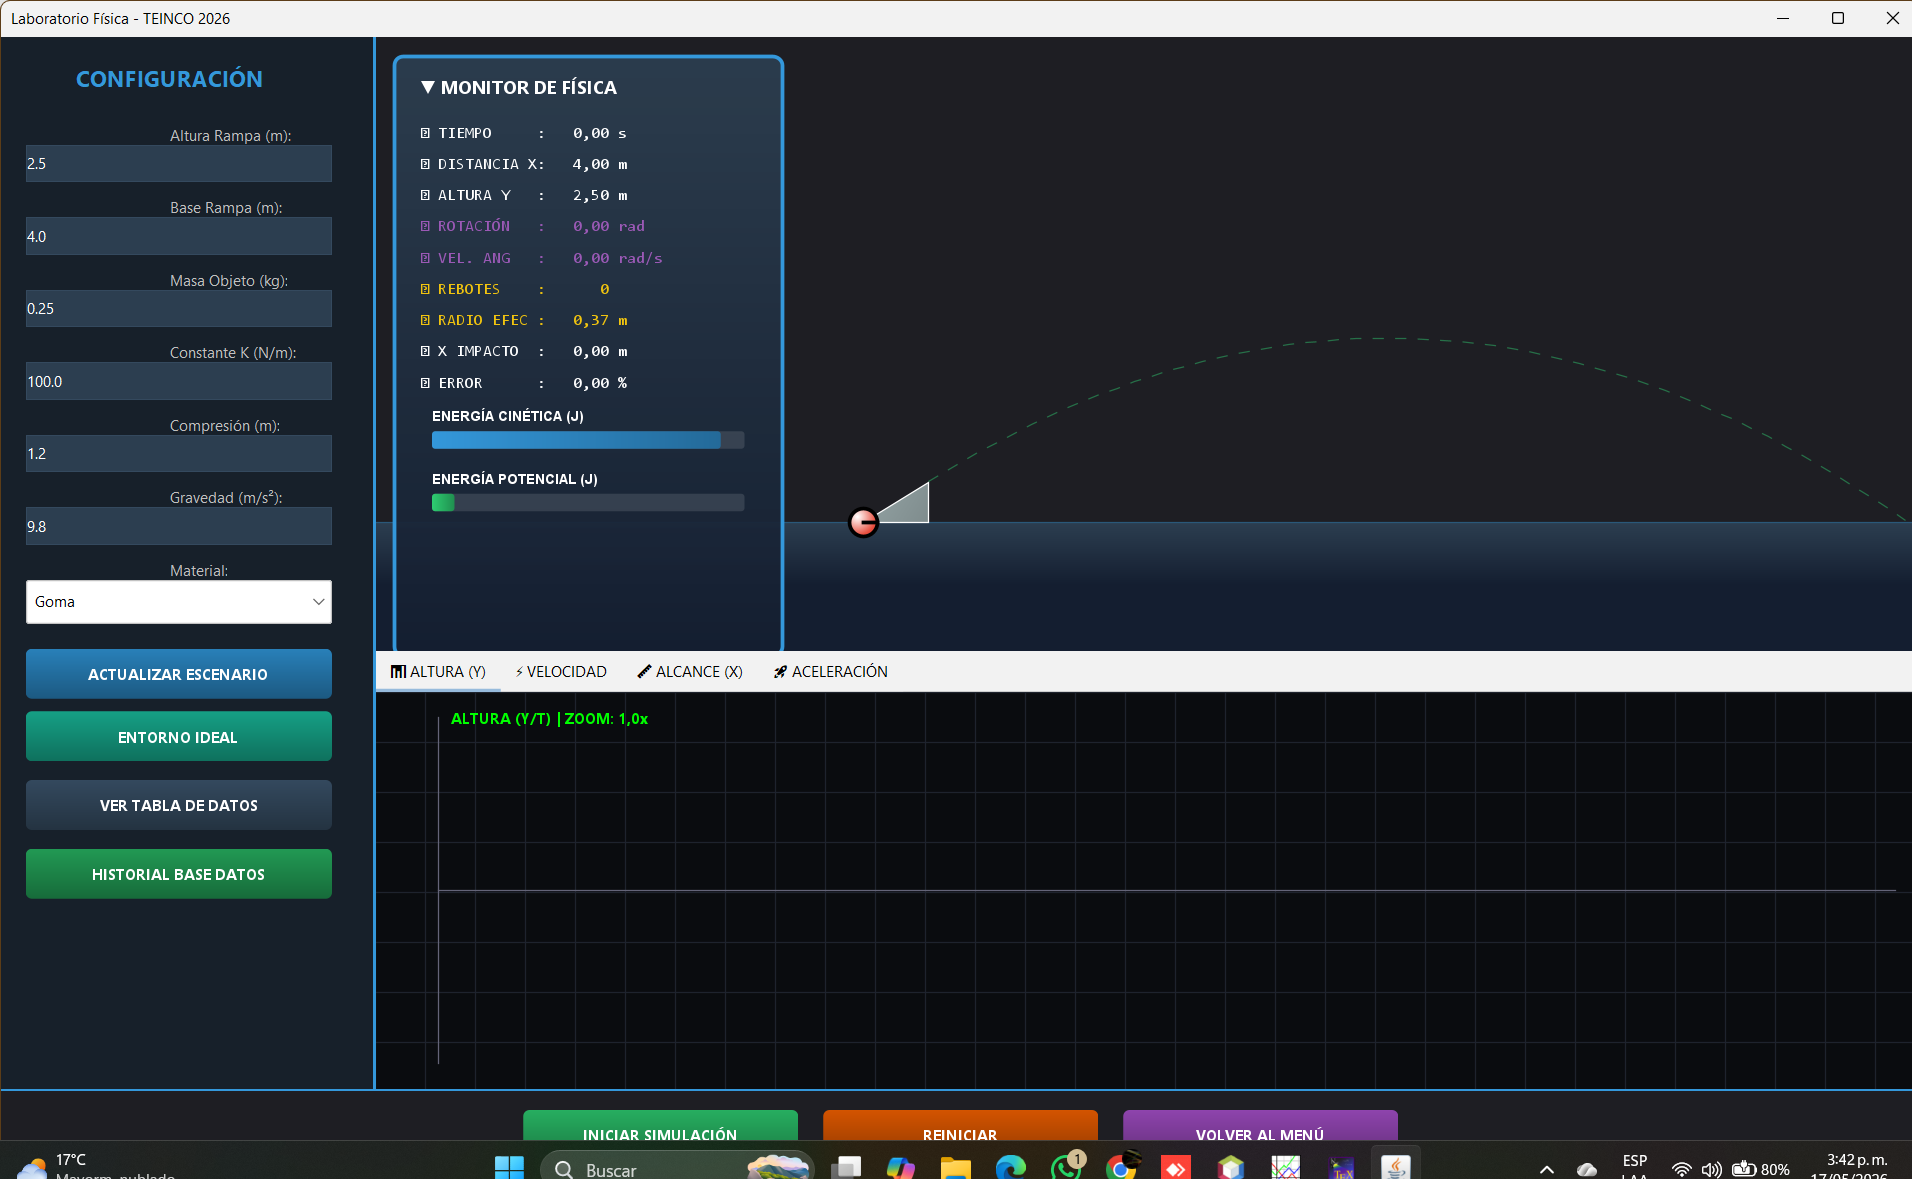
\includegraphics[width=0.7\textwidth]{parabola.png}
	\caption{Entorno gráfico del Módulo I para el desarrollador. Se muestra el renderizado dinámico de la trayectoria balística en el canvas principal y la actualización síncrona de los vectores de estado cinemático frente a la resistencia aerodinámica.}
	\label{fig:arquitectura_parabola}
\end{figure}
	\subsection{Discretización de Ecuaciones Diferenciales Acopladas}
	El estado dinámico del proyectil es gobernado en cada instante de tiempo por un vector de estado multidimensional $S = [x, y, v_x, v_y]^T$. El programador puede auditar la clase encargada del bucle de físicas, donde se resuelven iterativamente las derivadas temporales en función de una ventana infinitesimal discreta de tiempo (\textit{Time Step}) denotada como $\Delta t$:
	\begin{equation}
		v_{\text{magnitud}} = \sqrt{(v_x)^2 + (v_y)^2}
	\end{equation}
	\begin{equation}
		F_d = \frac{1}{2} C_d \cdot \rho \cdot A \cdot (v_{\text{magnitud}})^2
	\end{equation}
	Las componentes vectoriales de las fuerzas retardadoras se proyectan en sentido inverso a los cosenos y senos directores del movimiento instantáneo ($\cos\phi = v_x / v_{\text{magnitud}}$ y $\sin\phi = v_y / v_{\text{magnitud}}$), traduciéndose en el siguiente esquema de asignación algorítmica recursiva ejecutada en cada iteración del bucle:
	\begin{equation}
		v_x(t + \Delta t) = v_x(t) - \left( \frac{F_d \cdot v_x(t)}{m \cdot v_{\text{magnitud}}} \right) \Delta t
	\end{equation}
	\begin{equation}
		v_y(t + \Delta t) = v_y(t) - \left( g + \frac{F_d \cdot v_y(t)}{m \cdot v_{\text{magnitud}}} \right) \Delta t
	\end{equation}
	\begin{equation}
		x(t + \Delta t) = x(t) + v_x(t + \Delta t) \cdot \Delta t
	\end{equation}
	\begin{equation}
		y(t + \Delta t) = y(t) + v_y(t + \Delta t) \cdot \Delta t
	\end{equation}
	Este método actualiza las velocidades inmediatamente antes de calcular el desplazamiento de posición espacial, lo cual confiere al resolvedor una mayor estabilidad energética intrínseca frente al método de Euler simple estándar, mitigando la acumulación artificial de errores numéricos de truncamiento exponencial.
	
	\subsection{Estructura Lógica del Inicializador del Entorno Ideal}
	Cuando el programador analiza el controlador del botón \textbf{"Entorno Ideal"}, observará que el sistema intercepta el flujo, limpia las estructuras de listas dinámicas (\texttt{ArrayList<Point2D.Double>}) y sobreescribe de forma imperativa las variables mediante el siguiente fragmento estructurado:
	\begin{lstlisting}[language=Java]
		// Configuracion por contrato del Entorno Ideal en el Modulo I
		public void configurarEntornoIdeal() {
			this.alturaRampa = 2.0;
			this.baseRampa = 3.0;
			this.masaObjeto = 1.0;
			this.constanteK = 200.0;
			this.compresionResorte = 0.5;
			this.gravedad = 9.81;
			this.coeficienteFriccionRampa = 0.0; // Estado Hielo puro
			this.densidadAire = 0.0;             // Vacio absoluto
			this.isIdealActivated = true;
			
			// Forzar recalculo de matrices y dibujo estatico de la curva verde
			precalcularTrayectoriaAnaliticaGalileo();
			notificarCambioVista();
		}
	\end{lstlisting}
	
	\subsection{Inyección Arquitectónica del Catálogo de Materiales}
	Para el desarrollador de sistemas, el catálogo de materiales superficiales de la rampa está implementado a través de una enumeración estructurada (\texttt{enum MaterialType}). Cada elemento de la enumeración expone un atributo flotante inmutable correspondiente a su coeficiente dinámico de fricción real. Al momento de evaluar el deslizamiento inicial, la aceleración tangencial neta en la rampa se ve afectada directamente por la llamada polimórfica \texttt{MaterialType.getCoeficienteFriccion()}, simplificando la extensión de la plataforma mediante la adición de nuevos elementos sin modificar el motor cinemático.
	
	\subsection{Mapeo Gráfico del Motor de Parábolas}
	Para depurar el comportamiento visual de la renderización balística frente a las ecuaciones implementadas, el programador dispone del siguiente mapa de distribución de pantalla en el Módulo I:
	
	
	
	% ==========================================
	% SECCIÓN 4: MOTOR MATEMÁTICO DEL MÓDULO II (DESARROLLADOR)
	% ==========================================
	\section{Ingeniería del Movimiento Oscilatorio y Ley de Hooke}
	El Módulo II modela la física de un oscilador armónico unidimensional montado verticalmente. Desde la perspectiva del programador, este sistema representa la implementación práctica de una ecuación diferencial de segundo orden amortiguada y forzada mecánicamente por el medio viscoso.
	
	\subsection{Lógica de Flujo para Regímenes de Amortiguamiento}
	El resolvedor físico del muelle calcula antes del inicio del bucle el discriminante característico de la ecuación del oscilador ($\Delta = b^2 - 4 \cdot m \cdot k$). A través de una estructura de control de bifurcación condicional anidada (\texttt{if-else}), el motor altera el algoritmo de pintado y el cálculo de la envolvente exponencial en función del régimen dictaminado por las variables del sistema:
	\begin{itemize}
		\item \textbf{Subamortiguado ($\Delta < 0$):} Ejecuta funciones armónicas amortiguadas multiplicadas por el factor exponencial de decaimiento temporal $e^{-(\frac{b}{2m})t}$.
		\item \textbf{Críticamente Amortiguado ($\Delta = 0$):} El sistema converge con rapidez geométrica hacia la neutralidad espacial sin experimentar oscilaciones repetitivas.
		\item \textbf{Sobreamortiguado ($\Delta > 0$):} Resuelve el decaimiento mediante la suma de dos componentes exponenciales puras con coeficientes reales independientes.
	\end{itemize}
	
	\subsection{Abstracción de la Configuración Ideal del Oscilador}
	La activación de las condiciones ideales en el muelle realiza una mutación directa sobre las variables del modelo, anfractuando de forma absoluta el parámetro viscoso $b$ para dar paso a un ciclo infinito de oscilación limpia:
	\begin{lstlisting}[language=Java]
		// Inicializacion forzada del Oscilador Armonico Simple Libre
		public void inicializarMuelleIdeal() {
			this.constanteElasticidadK = 150.0;
			this.masaSuspendida = 0.5;
			this.elongacionInicialX0 = 0.8;
			this.coeficienteAmortiguamientoB = 0.0; // Anulacion de perdidas
			this.frecuenciaAngularNatural = Math.sqrt(k / m);
			this.periodoTeorico = (2.0 * Math.PI) / frecuenciaAngularNatural;
		}
	\end{lstlisting}
	
	\subsection{Algoritmo Paramétrico de Dibujo de la Geometría del Muelle}
	El resorte helicoidal visualizado en pantalla no es una secuencia de imágenes estáticas ni un recurso pre-renderizado. El programador implementó un generador paramétrico procedural de líneas elásticas. El algoritmo toma la longitud instantánea del resorte $L_{\text{instantánea}} = L_{\text{natural}} + x(t)$ y la divide equitativamente entre el número de espiras fijas parametrizadas. El bucle calcula coordenadas alternas en el eje horizontal X (simulando el ancho físico del alambre) mientras desplaza incrementalmente el eje Y, uniendo los nodos resultantes mediante el uso del método \texttt{graphics2D.drawPolyline()}. Esto permite que el resorte se estire o se contraiga de forma dinámica siguiendo fielmente los datos generados por el motor numérico.
	
	\subsection{Mapeo Gráfico del Motor de Oscilación}
	La verificación de la interfaz de desarrollo acoplada al renderizador procedimental del oscilador helicoidal se ilustra en el siguiente diagrama técnico de pantalla:
	
	\begin{figure}[htbp]
		\centering
		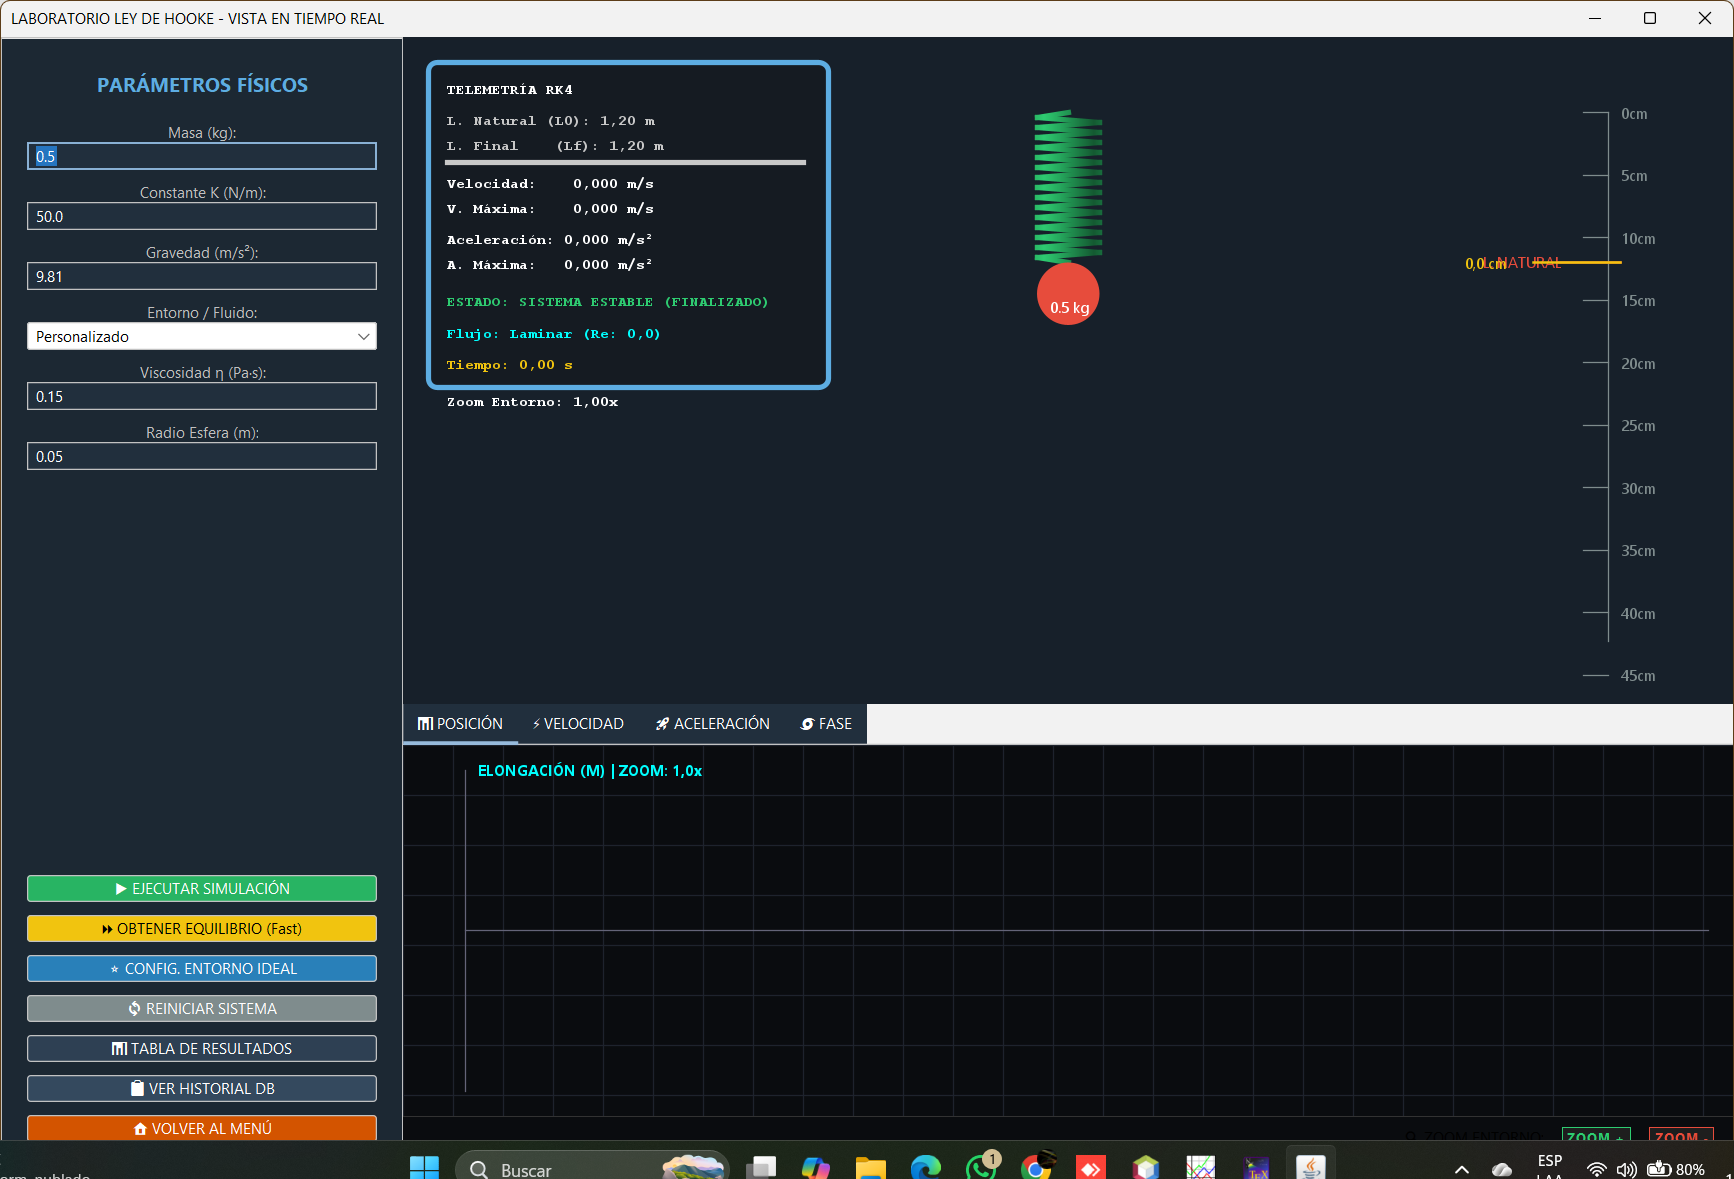
\includegraphics[width=0.7\textwidth]{resorte.png}
		\caption{Entorno gráfico del Módulo II para el desarrollador. Se muestra la sincronización en tiempo real entre la deformación del muelle y la inyección de la señal sinusoidal en el osciloscopio inferior.}
		\label{fig:arquitectura_resorte}
	\end{figure}% ==========================================
	% SECCIÓN 5: TELEMETRÍA Y LOGS DE DEPURACIÓN
	% ==========================================
	\section{Telemetría Avanzada, Métricas de Rendimiento y Logging}
	
	\subsection{Arquitectura de Captura en el Monitor HUD}
	El monitor de visualización frontal transparente o HUD está acoplado de forma desacoplada al backend a través de llamadas de notificación asíncronas. Desde la perspectiva de la codificación de software, la clase del HUD implementa un método observador que recibe copias inmutables del vector de estado cinemático en intervalos exactos de $\Delta t$. El desarrollador debe notar que para mantener la eficiencia de la GPU y evitar fugas de memoria por la creación excesiva de objetos de tipo \texttt{String}, los datos numéricos de velocidad angular ($\omega$), energía cinética traslacional ($E_k$), potencial elástica ($E_e$) y fuerzas elásticas instantáneas se formatean directamente utilizando estructuras fijas de almacenamiento de caracteres como buffer de datos (\texttt{StringBuilder}).
	
	\subsection{Auditoría de Errores Numéricos e Instrumentales}
	Al interrumpirse la ejecución por el cese dinámico del movimiento, el controlador del software invoca el método encapsulado de análisis de desviación instrumental. El programador implementó el cálculo del error porcentual contrastando el valor numérico flotante real devuelto por el resolvedor discreto frente al resultado analítico exacto esperado por las ecuaciones de Galileo o del M.A.S. ideal:
	\begin{lstlisting}[language=Java]
	// Rutina de calculo de desviacion instrumental de datos numericos
	public double calcularErrorInstrumental(double valorIdeal, double valorReal) {
		if (Math.abs(valorIdeal) < 1e-9) {
			return 0.0; // Prevenir indeterminaciones por division por cero
		}
		return (Math.abs(valorIdeal - valorReal) / valorIdeal) * 100.0;
	}
	\end{lstlisting}
	
	% ==========================================
	% SECCIÓN 6: CAPA DE PERSISTENCIA SQLITE 3
	% ==========================================
	\section{Arquitectura del Backend de Persistencia y Base de Datos}
	La conservación de los históricos de simulación se implementa localmente a través de un motor de bases de datos relacional ligero e inyectado de forma embebida compatible con la especificación \texttt{SQLite 3}.
	
	\subsection{Patrón de Diseño Singleton aplicado a la Gestión de Conexiones}
	Para impedir colisiones de acceso transaccional sobre el archivo físico de la base de datos local y evitar fugas de descriptores del sistema operativo por aperturas simultáneas de canales, la capa de acceso a datos implementa el patrón creacional \textit{Singleton}. La clase de infraestructura \texttt{ConexionDB} restringe su constructor a un ámbito estrictamente privado, exponiendo un único punto global de acceso controlado sincronizado para hilos:
	\begin{lstlisting}[language=Java]
	// Implementacion del Patron Singleton Seguro para Hilos en el Backend
	public class ConexionDB {
		private static ConexionDB instancia;
		private Connection conexion;
		
		private ConexionDB() {
			try {
				String url = "jdbc:sqlite:laboratorio_fisica.db";
				this.conexion = DriverManager.getConnection(url);
				inicializarTablas();
			} catch (SQLException e) {
				System.err.println("Error critico JDBC: " + e.getMessage());
			}
		}
		
		public static synchronized ConexionDB getInstancia() {
			if (instancia == null) {
				instancia = new ConexionDB();
			}
			return instancia;
		}
		
		public Connection getConexion() {
			return this.conexion;
		}
	}
	\end{lstlisting}
	
	\subsection{Manejo Asíncrono de Datos mediante SwingWorker}
	Para garantizar que la tasa de refresco del canvas gráfico principal no deciga ni experimente congelamientos visuales indeseados durante la lectura o escritura de datos históricos pesados sobre el almacenamiento local, el programador implementó operaciones asíncronas extendiendo la clase abstracta \texttt{javax.swing.SwingWorker<Void, Void>}. 
	
	El método \texttt{doInBackground()} se encarga de empaquetar de forma transparente los parámetros físicos de la simulación y de inyectarlos de forma transaccional mediante sentencias de inserción preparadas de SQL (\texttt{PreparedStatement}), anulando activamente vulnerabilidades de inyección de código. Al culminar de forma ese proceso en el hilo secundario de procesamiento, el despachador de eventos de Java invoca automáticamente el método de retorno \texttt{done()} sobre el hilo principal para actualizar la vista de la bitácora relacional (\texttt{JTable}) sin entorpecer la experiencia del usuario.
	
	% ==========================================
	% SECCIÓN 7: GLOSARIO TÉCNICO Y CONTROL DE ERRORES
	% ==========================================
	\section{Apéndice Técnico para Programadores y Desarrolladores}
	
	\subsection{Glosario de Abstracciones y Prácticas de Codificación}
	A continuación, se compendia el glosario de términos especializados utilizados en la arquitectura interna del sistema:
	\begin{description}
	\item[Bit-Blit:] Operación transaccional de gráficos por computadora que transfiere un bloque completo de bits de color desde una imagen en memoria hacia el buffer de pantalla visible de forma síncrona.
	\item[Double Buffering:] Estrategia gráfica implementada para precalculcar y dibujar los vectores en una imagen oculta en RAM, mitigando el parpadeo en las animaciones Swing.
	\item[Euler Modificado:] Algoritmo de integración de ecuaciones diferenciales que promedia las derivadas al inicio y al final del paso de tiempo $\Delta t$, otorgando estabilidad cinemática al sistema.
	\item[Race Condition:] Condición de carrera que ocurre cuando múltiples hilos intentan alterar simultáneamente el estado de una misma variable no protegida en la memoria compartida de la JVM.
	\item[SOLID:] Conjunto de cinco principios de diseño orientado a objetos destinados a crear arquitecturas de software más legibles, escalables y fáciles de mantener a largo plazo.
	\item[SQLite 3:] Motor relacional embebido que almacena la totalidad de la base de datos institucional en un único archivo plano sin requerir puertos de red activos.
	\item[SwingWorker:] Clase utilitaria de Java diseñada para ejecutar tareas pesadas de entrada y salida en hilos secundarios de background, retornando los resultados de forma segura a la interfaz gráfica.
	\end{description}
	
	\subsection{Matriz de Control de Alertas del Backend}
	El programador dispone de la siguiente matriz técnica estandarizada para el rastreo y la gestión de excepciones lógicas capturadas por los bloques \texttt{try-catch} del sistema (las celdas largas han sido segmentadas mediante columnas de ancho fijo \texttt{p\{width\}} para evitar desbordamientos de caja):
	
	\begin{table}[htbp]
	\centering
	\caption{Códigos de Control de Excepciones Técnicas e Invariantes del Código.}
	\begin{tabular}{lp{6cm}l}
		\toprule
		\textbf{Excepción} & \textbf{Estrategia de Captura e Intercepción} & \textbf{Impacto en el Sistema} \\
		\midrule
		\texttt{SQLException} & Registro en logs de consola y cierre preventivo de cursores SQL abiertos. & Falla en persistencia histórica. \\
		\texttt{NullPointer} & Validación previa contractual del estado de los vectores mediante \texttt{assert}. & Detención preventiva del motor. \\
		\texttt{Arithmetic} & Filtrado estricto de valores de entrada flotantes en los campos JTextfield. & Evita indeterminaciones. \\
		\bottomrule
	\end{tabular}
	\label{tab:excepciones_backend}
	\end{table}
	
	% ==========================================
	% BIBLIOGRAFÍA FORMAL PARA INGENIERÍA DE SOFTWARE
	% ==========================================
	\section{Referencias Bibliográficas y Fuentes de Ingeniería}
	La infraestructura de código, patrones y resolvedores numéricos de este sistema se sustentan sobre la base teórica de las siguientes publicaciones científicas:
	
	\begin{enumerate}[label={[ \arabic* ]}]
	\item Schildt, H. (2020). \textit{Java: The Complete Reference}. 11va Edición. McGraw-Hill Education.
	\item Gamma, E., Helm, R., Johnson, R., \& Vlissides, J. (1994). \textit{Design Patterns: Elements of Reusable Object-Oriented Software}. Addison-Wesley.
	\item Serway, R. A., \& Jewett, J. W. (2018). \textit{Física para Ciencias e Ingeniería}. Vol. 1. 10ma Edición. Cengage Learning.
	\item Elmasri, R., \& Navathe, S. (2016). \textit{Fundamentos de Sistemas de Bases de Datos}. 7ma Edición. Pearson Educación.
	\end{enumerate}
	
\end{document}
